\documentclass[a4paper,10pt]{report}

\usepackage{graphicx}
\usepackage{color}

\usepackage{caption}
\usepackage{subcaption}

\usepackage[portuguese]{babel}
\usepackage[utf8]{inputenc}
\usepackage[T1]{fontenc}

\usepackage{geometry}
\geometry{a4paper}
\usepackage[parfill]{parskip}

\usepackage{changepage}

\usepackage{amsmath}

\usepackage{fancyhdr}

\usepackage{nopageno}

\graphicspath{{./imagens/}}

\usepackage{url}

\usepackage{verbatim}
\usepackage{fancyvrb}
\usepackage{listings}
\usepackage{float}

\usepackage[colorlinks=true,linkcolor=blue,citecolor=blue]{hyperref}


\lstset{
    extendedchars=\true,
    inputencoding=utf8
}

\renewcommand{\lstlistingname}{Código}
\usepackage{color}
\definecolor{grey}{rgb}{0.9,0.9,0.9}
\definecolor{greyD}{rgb}{0.5,0.5,0.5}

\lstnewenvironment{code}[1][]%
{
   \noindent
   \lstset{
  float=htpb,
  backgroundcolor=\color{grey},
  basicstyle=\scriptsize,
  numbers=left,
  numbersep=5pt,
  numberstyle=\tiny\color{greyD},
  breaklines=true,
  frame=single,
  #1}
}
{}

\begin{document}

\begin{titlepage}
\begin{center}

\begin{flushleft}

\includegraphics[height=3.00cm]{EENG.jpg}\\
\end{flushleft}

\vspace{1.5cm}

\Large{\textbf{LEI --- Licenciatura de Engenharia Informática}}\\
\vspace{1cm}
\Large{\textbf{Processamento de Linguagens}}\\

\vspace{1cm}

\Huge{\textbf{Compilador de uma LPIS}} \\

\vspace{2cm}

\Large{\textbf{Orlando Costa -  a67705, Paulo Araujo - a58925, Rui Oliveira - a67661}}\\
\begin{figure}[h]
\centering
\begin{subfigure}{.3\textwidth}
  \centering
  
\includegraphics[width=\textwidth]{Orlando.jpg}
\end{subfigure}
\begin{subfigure}{.3\textwidth}
  \centering
  
\includegraphics[width=\textwidth]{Paulo.jpg}
\end{subfigure}
\begin{subfigure}{.3\textwidth}
  \centering
  
\includegraphics[width=\textwidth]{Oliveira.jpg}
\end{subfigure}
\end{figure}

\vspace{1.5cm}
Braga, 7 de Junho de 2015

\end{center}

\end{titlepage}


\begin{abstract}
Este relatório descreve a resolução de um conjunto de exercícios propostos, que consistem no desenvolvimento de programas na linguagem C com o auxílio de geradores de filtros de texto, como o Flex. Para cada problema é realizada uma breve análise sobre o trabalho efetuado, as decisões que lideraram o seu desenvolvimento e as estruturas implementadas, assim como uma explicação do seu funcionamento. 

Os problemas resolvidos consistem no desenvolvimento de filtros de texto que:
\begin{itemize}
\item processa um ficheiro XML com descrições de fotografias e gera um álbum HTML.
\item processa de um ficheiro XML anotado com tags Enamex e gera páginas HTML apresentando as "pessoas", "países", "cidades" e organizações nele identificadas. 
\item processa vários ficheiros de texto, compostos por letras de canções, e gera documentos em LATEX para cada uma delas.
\end{itemize}
Para cada problema é apresentado o código em linguagem C e as expressões regulares desenvolvidas, sendo estes suportados por exemplos e devidos resultados.
\end{abstract}
%----------------------------------------------------------------------
%\newpage
%\phantom{placeholder} % doesn't appear on page
%\thispagestyle{empty} % if want no header/footer
%----------------------------------------------------------------------
\tableofcontents
%\phantom{placeholder} % doesn't appear on page
\thispagestyle{empty} % if want no header/footer
%----------------------------------------------------------------------
%\newpage
%\phantom{placeholder} % doesn't appear on page
%\thispagestyle{empty} % if want no header/footer
%----------------------------------------------------------------------
%\pagestyle{fancy}
%\setlength{\headheight}{15.2pt}
%\fancyhf{} % apagar as configurações actuais
%\fancyfoot[LE,RO]{\thepage}
%\fancyhead[LE,RO]{PL - Trabalho Pratico 1 --- Araujo P., Belo O., Oliveira R.}
%\page{setcounter}{0}
%----------------------------------------------------------------------

\chapter{Introdução}
\label{cap:intro}
O presente trabalho enquadra-se na unidade curricular de Processamento de Linguangens da Licenciatura em Engenharia Informática da Universidade do Minho. O trabalho pretende aumentar a experiência em engenharia de linguagens, 

\section{Linguagem de programação imperativa simples}
    Previamente ao desenvolvimento do compilador existe a necessidade de definir uma linguagem sobre a qual este atua, com base numa qualquer linguagem imperativa. Neste sentido e por simplicidade e familiaridade, a linguagem de programação C é a selecionada. Esta linguagem foi simplificada por forma a adaptar-se aos requisitos propostos, sofrendo as seguinte modificações na sua estrutura:

    - Apenas permite manusear variáveis do tipo inteiro (escalar ou array).
    - Suporta apenas as instruções vulgares de controlo de fluxo de execução (condicional e cíclica), tais como if-else, for, while e do-while.
    - As instruções que controlam inserção e output de valores (tipicamente printf e scanf) estão adaptadas para suportar apenas inteiros, e então estão renomeadas (printi e scani).
    - As expressões lógicas devem estar rodeadas por parentises para facilitar a sua distinção e ordem quando em conjunto com expressões aritméticas. 


    <Programa exemplo (programa exemplo que mostre de forma simples todas as funcionalidades - funçoes, atribuiçoes, ciclos, expressoes logicas e aritmeticas)> 

\section{Arquitetura}
    O sistema desenvolvido é constituído por 2 principais modelos:  parser.l, compiler.y, que são respetivamente o analisador léxico e analisador sintático. 

    Na Figura \ref{fig:dependencias}, podemos ver as dependências dos ficheiros entre si.

    O analisador sintático, utiliza o ficheiro vmCompiler.h, este modulo é o responsável pelo tratamento das variáveis e funções existentes.

    Em vmCompiler.h podem-se fazer ações tais como adicionar uma variável, e consultar as variáveis existentes.

    O Sistema também usou duas estruturas de dados: um HashMap e ou Stack, hashmap utilizado para guardar as variáveis e as funções. A stack para na compilação controlar as label's dos ciclos.

    Na figura \ref{fig:struct}, pode-se ver as estruturas utilizadas em vmCompiler:
    \begin{itemize}
      \item Scope - têm uma map com a informação das variáveis, onde a chave é nome da variável e o valor é um EntryVar;
      \item EntryFun - guarda a informação sobre o tipo de uma função (argumentos de entrada e tipo de retorno);
      \item EntryVar - guarda o tipo, nome o endereço relativo de uma dada variável;
    \end{itemize}

    Com as estruturas anteriores em mente, as variáveis criadas em vmCompiler são as representadas na figura \ref{fig:objs}, onde pode-se ver duas variáveis do tipo Scope uma para o contexto global outra para o contexto interior a uma função.

    Existe uma map de EntryFun (mFuncMap) onde a chave é o nome da função.
    
    A variável DecFunAux, é um apontador temporário para um função que se esteja a declarar.

\begin{figure}
\centering
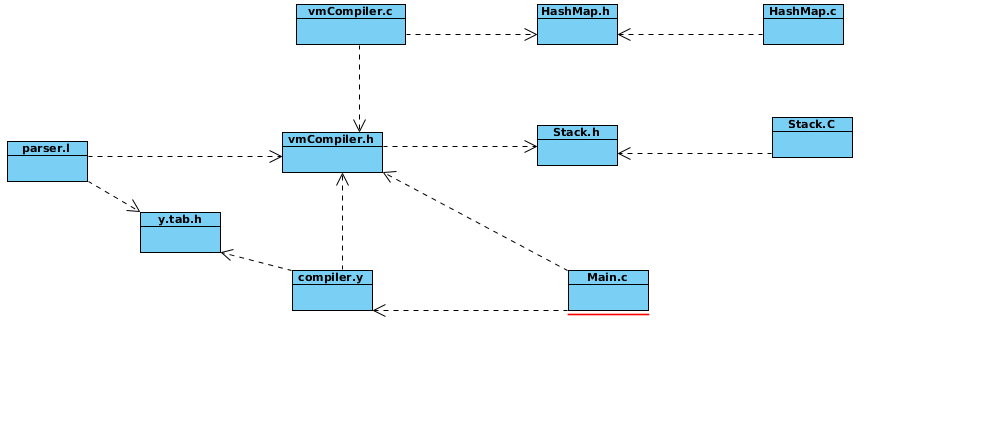
\includegraphics[width=15cm]{imagens/dependecias.png}
\caption{Diagrama das pedendencias dos ficheiros}
\label{fig:dependencias}
\end{figure}

\begin{figure}
\centering
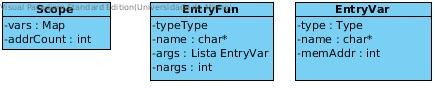
\includegraphics[width=10cm]{imagens/estruturas.jpg}
\caption{Diagrama das estruturas usadas em vmCompiler}
\label{fig:struct}
\end{figure}

\begin{figure}
\centering
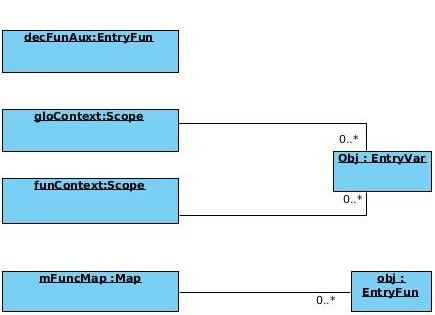
\includegraphics[width=10cm]{imagens/objetos.jpg}
\caption{Diagrama dos objetos existente em vmCompiler}
\label{fig:objs}
\end{figure}



\section{Estruturas de dados}

\subsection{Stack}
      De forma a evitar confusão na atribuição de \emph{labels} relativas a \emph{ifs} e \emph{loops} é utilizado um contador de condições. À medida que é encontrada uma instrução que implique o uso de uma condição, este contador é incrementado e o seu valor é colocado numa stack. Deste modo, o valor que se encontra no topo da stack é relativo ao último \emph{ciclo/if} encontrado. Sempre que é encontrado o final de uma condição, o valor no topo da stack é removido. Através do uso de um contador e de uma stack, é muito mais simples de gerir as \emph{labels} e as operações de controlo, como \emph{JUMPs} e \emph{JZs}.

\subsection{HashMap}



\chapter{Compilador}


\section{Analisador léxico}
  O analisador léxico construido deteta todos os símbolos terminais da linguagem (palavras reservadas, sinais e variáveis).
  É de se destacar a deteção de comentários, que são ignorados.
  De forma a que fosse mais fácil detetar os erros de sintaxe, o parser conta as linhas que já interpretou. Desta forma o analisador sintático quando dá erro diz a linha onde o erro aconteceu.  
  Para passar valores como o nome de variaveis ou números utiliza-se o yylval.


\section{Analalisador sintatico/semantico}

\section{Geração de codigo máquina}
    A cada regra da gramática, associamos acções a serem executadas à medida que estas são reconhecidas. Assim sendo, é feita uma tradução da linguagem desenvolvida para a linguagem \emph{assembly} da VM, à medida que cada instrução ou expressão é identificada. A maioria destas acções implica uma instrução de escrita no ficheiro de output. 


\chapter{Testes}


\chapter{Conclusão}
\label{cap:intro}
Terminado o desenvolvimento do trabalho, é importante referir que o mesmo nos permitiu aprofundar o conhecimento acerca do Gerador Léxico Flex assim como da análise léxica no geral, obrigando-nos também a utilizar ferramentas tais como HTML e Latex.\\
Relativamente ao problema do "Museu da Pessoa", a dificuldade recaiu na definição da estrutura de suporte de dados, dado que devido à falta de claridade do enunciado foi necessário re-implementar a estrutura de forma a que esta admitisse a funcionalidade de ter um índice geral em HTML.\\
No problema de "Processamento de Entidades Nomeadas" foi necessário chegar a um consenso acerca das tags que deveriam ser validadas e o relacionamento possível que estas teriam entre si. Após essa decisão, o desenvolvimento da estrutura que suporta esta informação tornou-se relativamente simples.\\
O problema "Processamento de Ficheiros com Canções" foi resolvida através da implementação de uma estrutura capaz de evitar que a ordem dos dados no ficheiro não seja significativa (e então armazena em memória a informação). A presença de certos elementos em datasets mais diversos (tais como header's não esperados e anotações em músicas) deram origem a problemas, sendo que a solução consistiu em ignorar essa informação. \\
Cada elemento do grupo realizou um exercício do enunciado proposto, apoiando-se mutuamente na existência de dificuldades. Apesar das dificuldades iniciais, encontramos-nos satisfeitos com o resultado final e estamos confiantes para o próximo trabalho.

\chapter{Anexos}
\label{cap:anex}


\section{Museu da Pessoa — tratamento de fotografias}
\label{seq:anex-museu}

\subsection{Filtro de Texto}
\label{seq:anex-museu-filtro}
\verbatiminput{anexos/2-1/C/parte_lex.l}

\subsection{Estrutura de dados}
\label{seq:anex-museu-est}
\lstinputlisting[language=c]{anexos/2-1/C/album.c}

\subsection{Cabeçalho ficheiro C}
\label{seq:anex-museu-header}
\lstinputlisting[language=c]{anexos/2-1/C/album.h}

\subsection{Testes}
\label{seq:anex-museu-test}
\subsubsection{Input teste 1}
\label{seq:anex-museu-test-in01}
\lstinputlisting[language=xml]{anexos/2-1/Exemplo1/legenda.xml}

\subsubsection{Output teste 1}
\label{seq:anex-museu-test-out01-01}
\lstinputlisting[language=html]{anexos/2-1/Exemplo1/AlbumGerado.html}

\begin{figure}[H]
\centering

\includegraphics[width=15cm]{anexos/2-1/Exemplo1/Screenshots/indice.png}
\caption{Indice HTML gerado pelo ficheiro XML}
\end{figure}

\label{seq:anex-museu-test-out01-02}
\lstinputlisting[language=html]{anexos/2-1/Exemplo1/1.html}

\begin{figure}[H]
\centering
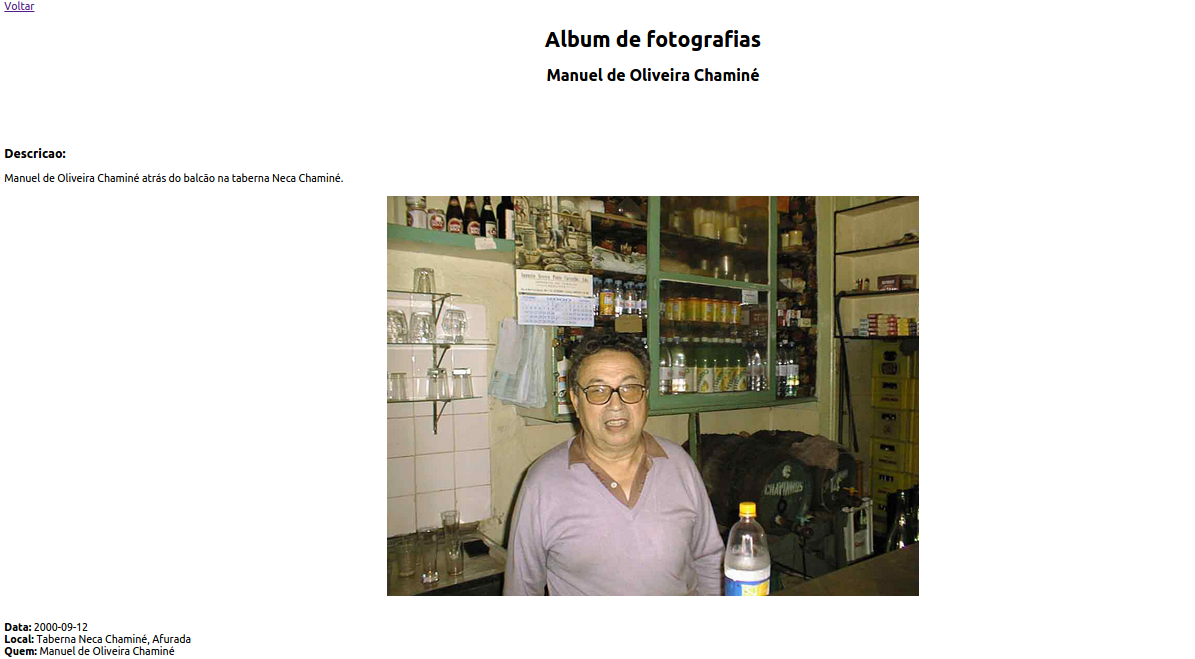
\includegraphics[width=15cm]{anexos/2-1/Exemplo1/Screenshots/pag1.png}
\caption{Pagina HTML gerada pelo ficheiro XML (1 de 2)}
\end{figure}

\begin{figure}[H]
\centering
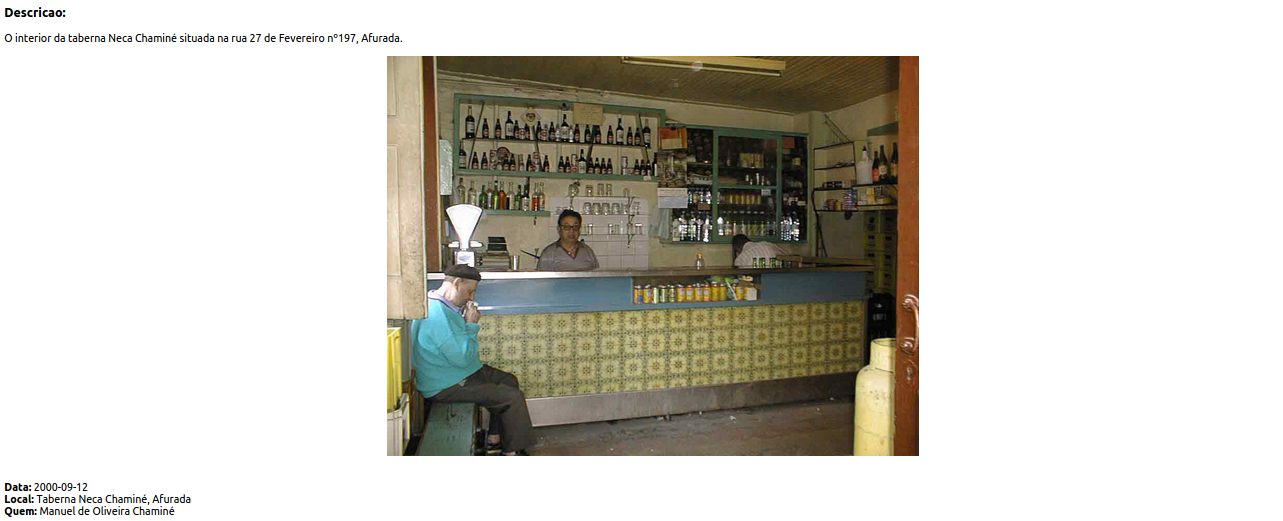
\includegraphics[width=15cm]{anexos/2-1/Exemplo1/Screenshots/pag2.png}
\caption{Pagina HTML gerada pelo ficheiro XML (2 de 2)}
\end{figure}

\subsubsection{Input teste 2}
\label{seq:anex-museu-test-in02}
\lstinputlisting[language=xml]{anexos/2-1/Exemplo2/legenda.xml}

\subsubsection{Output teste 2}
\label{seq:anex-museu-test-out02-01}
\lstinputlisting[language=html]{anexos/2-1/Exemplo2/AlbumGerado.html}

\begin{figure}[H]
\centering

\includegraphics[width=15cm]{anexos/2-1/Exemplo2/Screenshots/indice.png}
\caption{Indice HTML gerado pelo ficheiro XML}
\end{figure}

\label{seq:anex-museu-test-out02-02}
\lstinputlisting[language=html]{anexos/2-1/Exemplo2/5.html}

\begin{figure}[H]
\centering
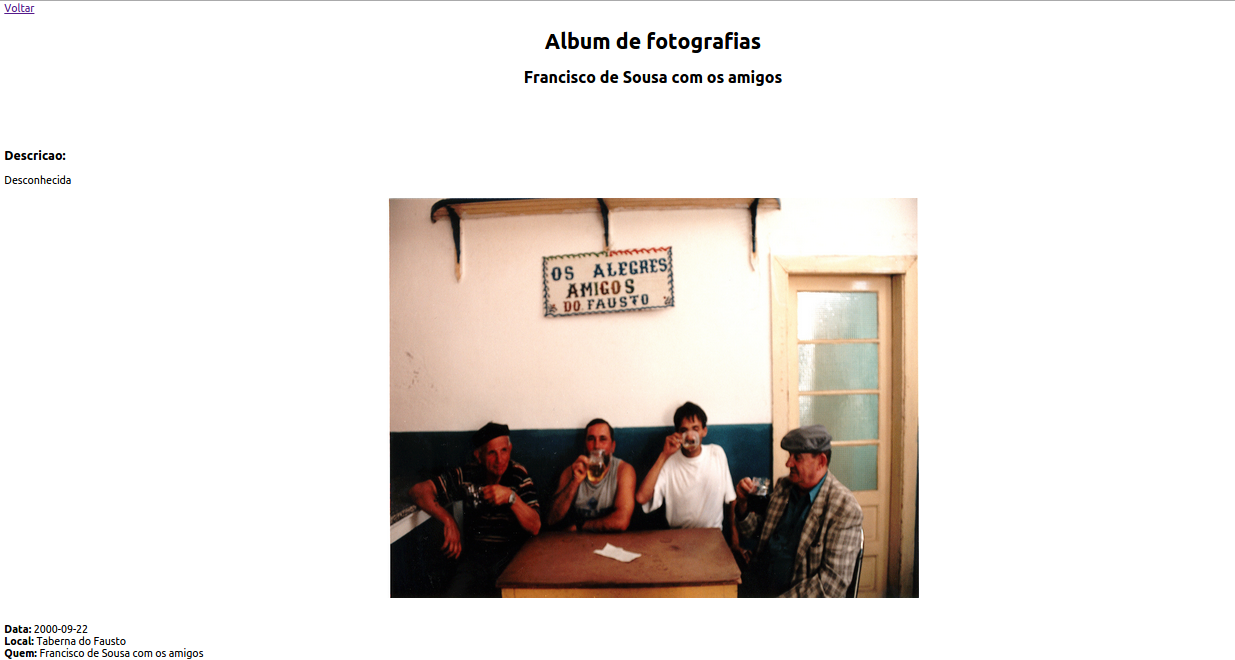
\includegraphics[width=15cm]{anexos/2-1/Exemplo2/Screenshots/pag1.png}
\caption{Pagina HTML gerada pelo ficheiro XML}
\end{figure}

\label{seq:anex-museu-test-out02-03}
\lstinputlisting[language=html]{anexos/2-1/Exemplo2/6.html}

\begin{figure}[H]
\centering
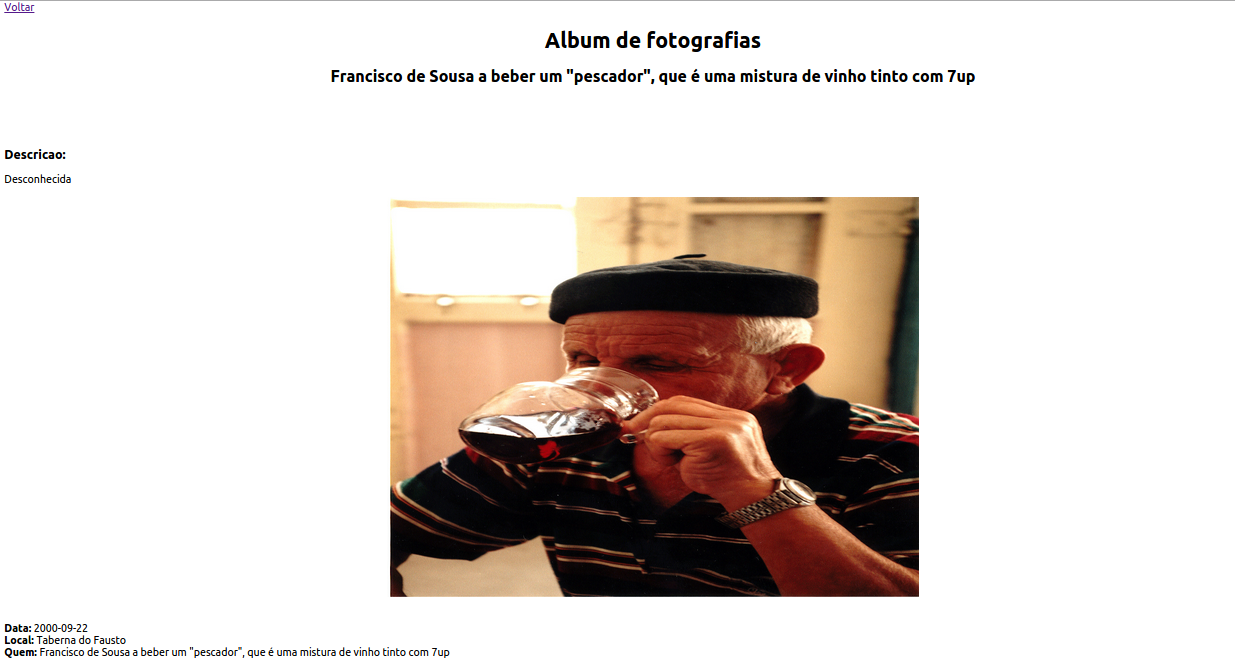
\includegraphics[width=15cm]{anexos/2-1/Exemplo2/Screenshots/pag2.png}
\caption{Pagina HTML gerada pelo ficheiro XML}
\end{figure}

\subsubsection{Input teste 3}
\label{seq:anex-museu-test-in03}
\lstinputlisting[language=xml]{anexos/2-1/Exemplo3/legenda.xml}

\subsubsection{Output teste 3}
\label{seq:anex-museu-test-out03-01}
\lstinputlisting[language=html]{anexos/2-1/Exemplo3/AlbumGerado.html}

\begin{figure}[H]
\centering

\includegraphics[width=15cm]{anexos/2-1/Exemplo3/Screenshots/indice.png}
\caption{Indice HTML gerado pelo ficheiro XML}
\end{figure}

\label{seq:anex-museu-test-out03-02}
\lstinputlisting[language=html]{anexos/2-1/Exemplo3/3.html}

\begin{figure}[H]
\centering
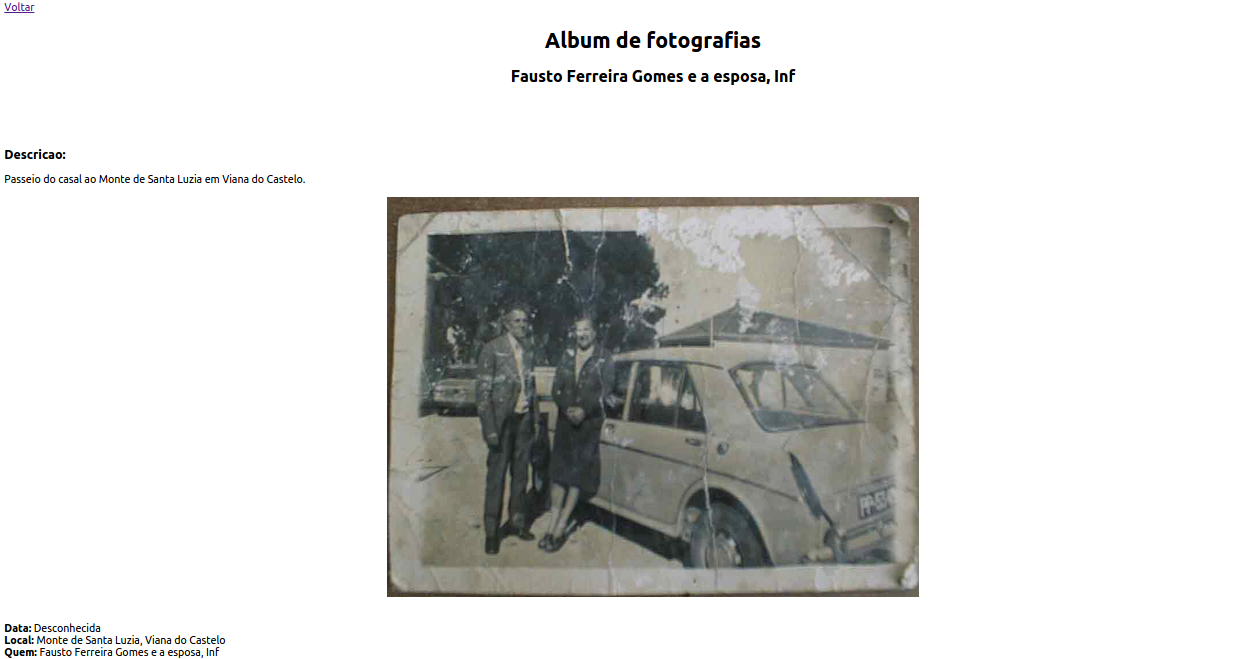
\includegraphics[width=15cm]{anexos/2-1/Exemplo3/Screenshots/pag2.png}
\caption{Pagina HTML gerada pelo ficheiro XML}
\end{figure}

\label{seq:anex-museu-test-out03-03}
\lstinputlisting[language=html]{anexos/2-1/Exemplo3/4.html}

\begin{figure}[H]
\centering
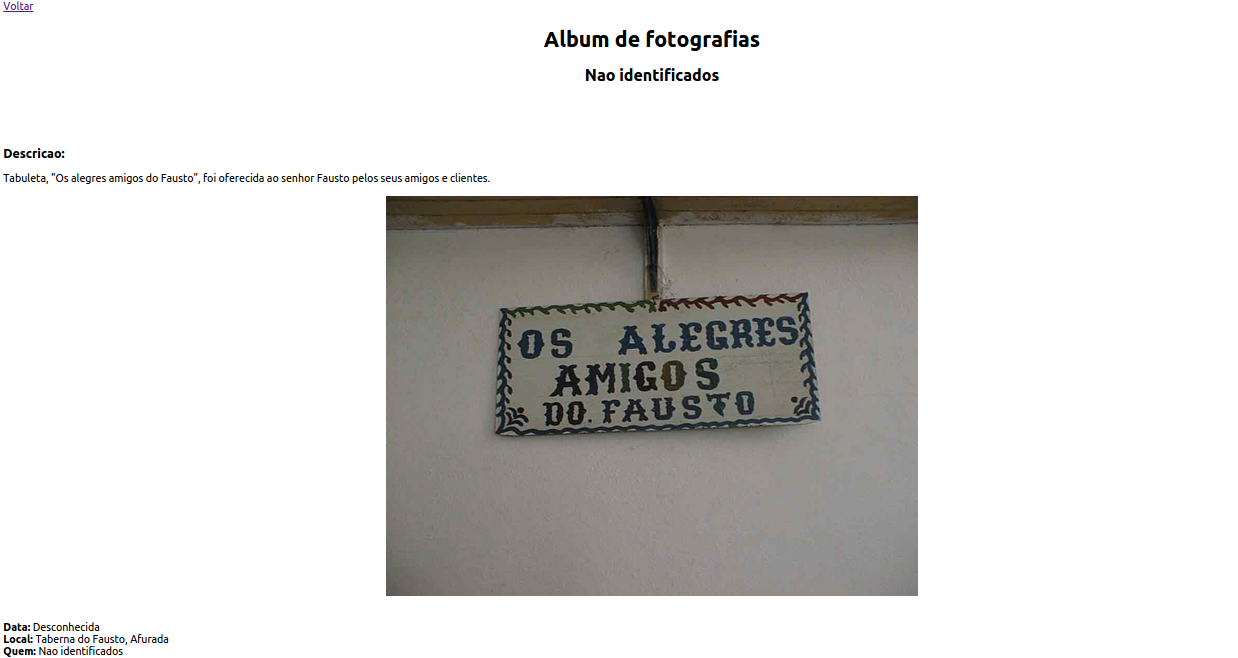
\includegraphics[width=15cm]{anexos/2-1/Exemplo3/Screenshots/pag1.png}
\caption{Pagina HTML gerada pelo ficheiro XML}
\end{figure}

\subsubsection{Input teste 4}
\label{seq:anex-museu-test-in04}
\lstinputlisting[language=xml]{anexos/2-1/Exemplo4/exemplo.xml}

\subsubsection{Output teste 4}
\label{seq:anex-museu-test-out04-01}
\lstinputlisting[language=html]{anexos/2-1/Exemplo4/AlbumGerado.html}

\begin{figure}[H]
\centering

\includegraphics[width=15cm]{anexos/2-1/Exemplo4/Screenshots/indice.png}
\caption{Indice HTML gerado pelo ficheiro XML}
\end{figure}

\label{seq:anex-museu-test-out04-02}
\lstinputlisting[language=html]{anexos/2-1/Exemplo4/1.html}

\begin{figure}[H]
\centering
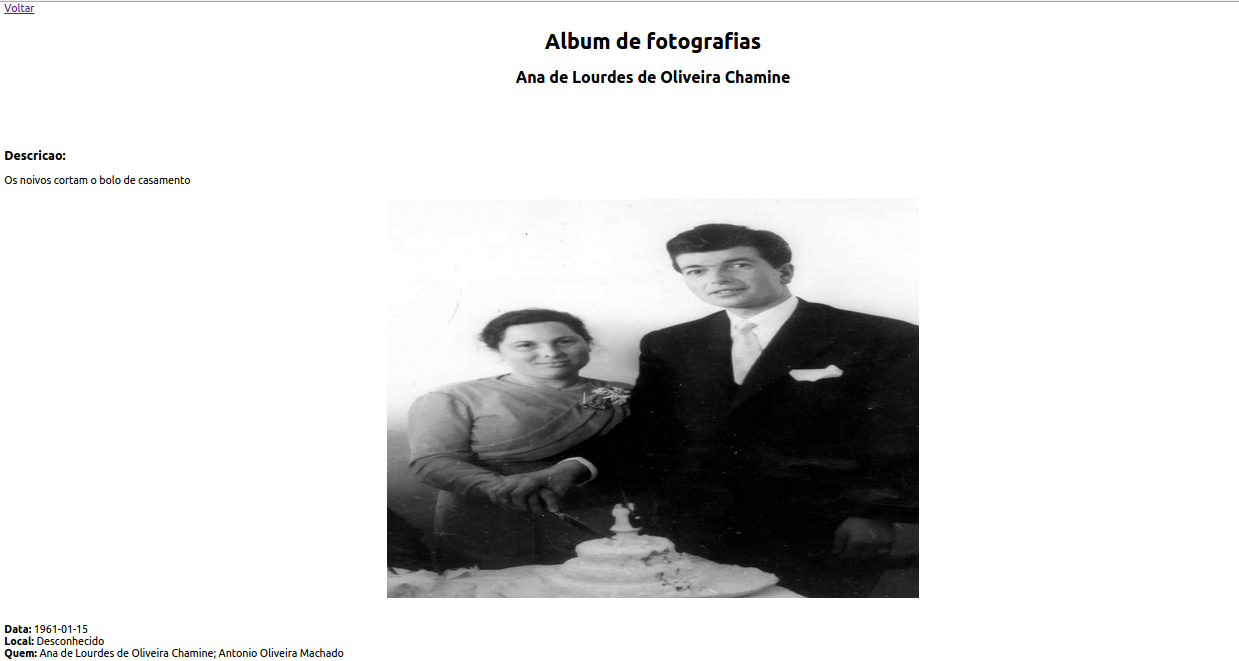
\includegraphics[width=15cm]{anexos/2-1/Exemplo4/Screenshots/pag1.png}
\caption{Pagina HTML gerada pelo ficheiro XML}
\end{figure}

\label{seq:anex-museu-test-out04-03}
\lstinputlisting[language=html]{anexos/2-1/Exemplo4/2.html}

\begin{figure}[H]
\centering
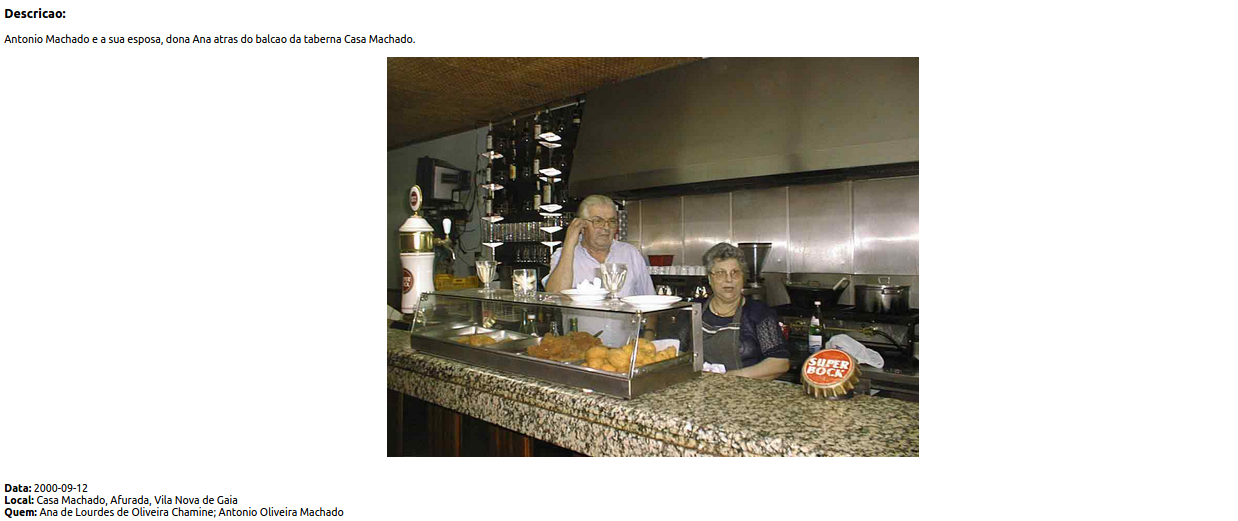
\includegraphics[width=15cm]{anexos/2-1/Exemplo4/Screenshots/pag2_2.png}
\caption{Pagina HTML gerada pelo ficheiro XML}
\end{figure}

\section{Processamento de Entidades Nomeadas (Enamex)}
\label{seq:anex-enamex}

\subsection{Filtro de Texto}
\label{seq:anex-enamex-filtro}
\verbatiminput{anexos/2-2/enamex.l}

\subsection{Estrutura de dados}
\label{seq:anex-enamex-est}
\lstinputlisting[language=c]{anexos/2-2/tree.c}

\subsection{Cabeçalho ficheiro C}
\label{seq:anex-enamex-header}
\lstinputlisting[language=c]{anexos/2-2/tree.h}


\subsection{Testes}
\label{seq:anex-enamex-test}
\subsubsection{Input teste 1}
\label{seq:anex-enamex-test-in01}
\lstinputlisting[language=xml,breaklines=true]{anexos/2-2/teste1_locais.txt}

\subsubsection{Output teste 1}
\label{seq:anex-enamex-test-out01}
\verbatiminput{anexos/2-2/2-5-a-out}
\begin{figure}[H]
\centering
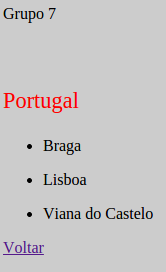
\includegraphics[width=4cm]{anexos/2-2/output_teste1.png}
\end{figure}


\subsubsection{Input teste 2}
\label{seq:anex-enamex-test-in02}
\lstinputlisting[language=xml,breaklines=true]{anexos/2-2/teste2_enunciado.txt}

\subsubsection{Output teste 2}
\label{seq:anex-enamex-test-out02}
\verbatiminput{anexos/2-2/2-5-a-out}
\begin{figure}[H]
\centering
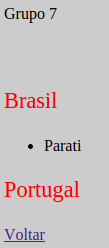
\includegraphics[width=4cm]{anexos/2-2/output_teste2.png}
\end{figure}

\subsubsection{Input teste 3}
\label{seq:anex-enamex-test-in03}
\lstinputlisting[language=xml,breaklines=true]{anexos/2-2/teste3_internet.txt}

\subsubsection{Output teste 3}
\label{seq:anex-enamex-test-out03}
\verbatiminput{anexos/2-2/2-5-a-out}
\begin{figure}[H]
\centering
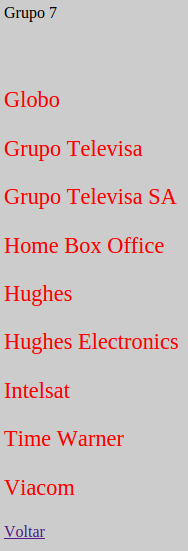
\includegraphics[width=4cm]{anexos/2-2/output_teste3.png}
\end{figure}






\section{Processamento de ficheiros com Canções}
\label{seq:anex-music}

\subsection{Filtro de Texto}
\label{seq:anex-music-filtro}
\verbatiminput{anexos/2-5/flex.l}

\subsection{Estrutura de dados}
\label{seq:anex-music-est}
\lstinputlisting[language=c]{anexos/2-5/musica.c}

\subsection{Cabeçalho ficheiro C}
\label{seq:anex-music-header}
\lstinputlisting[language=c]{anexos/2-5/musica.h}

\subsection{Testes}
\label{seq:anex-music-tests}
\subsubsection{Input teste 1}
\label{seq:anex-music-test-in01}
\verbatiminput{anexos/2-5/2-5-a-in}

\subsubsection{Output teste 1}
\label{seq:anex-music-test-out01}
\verbatiminput{anexos/2-5/2-5-a-out}

\subsubsection{Input teste 2}
\label{seq:anex-music-test-in02}
\verbatiminput{anexos/2-5/2-5-a-in}

\subsubsection{Output teste 2}
\label{seq:anex-music-test-out02}
\verbatiminput{anexos/2-5/2-5-b-out}

\subsubsection{Input teste 3}
\label{seq:anex-music-test-in03}
\verbatiminput{anexos/2-5/2-5-c-in}

\subsubsection{Output teste 3}
\label{seq:anex-music-test-out03}
\verbatiminput{anexos/2-5/2-5-c-out}

\begin{figure}
\centering
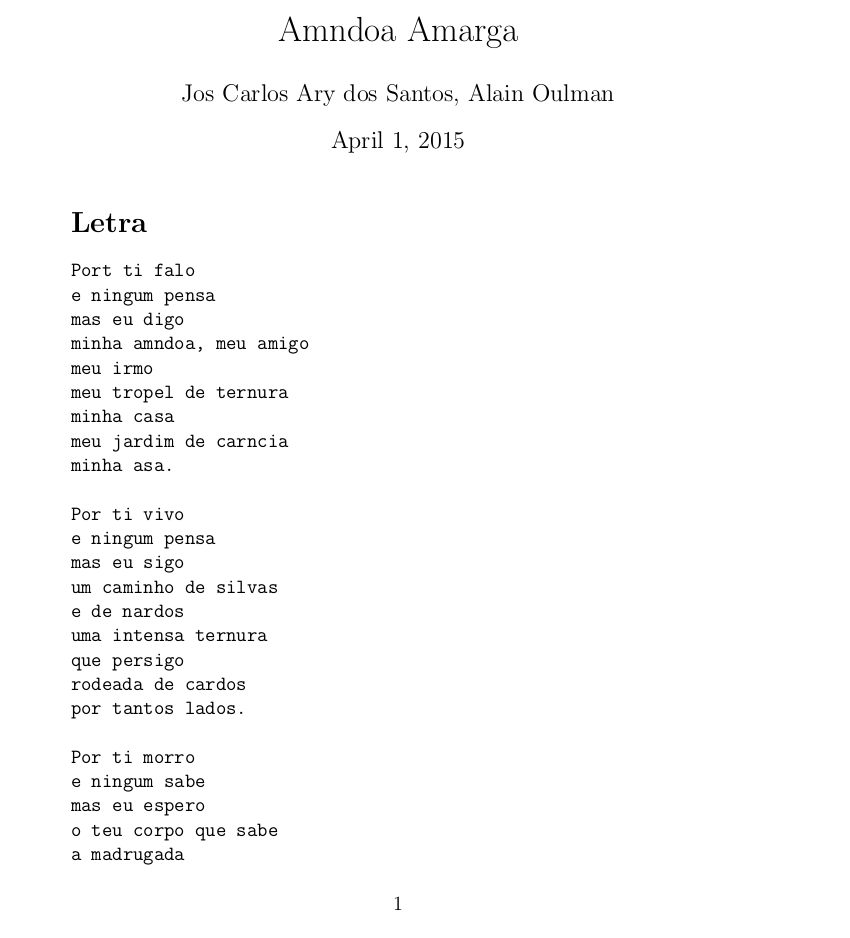
\includegraphics[width=15cm]{anexos/2-5/2-5-a-img1.png}
\caption{PDF gerado por o ficheiro latex (teste 1). Pagina 1 de 2}
\end{figure}

\begin{figure}
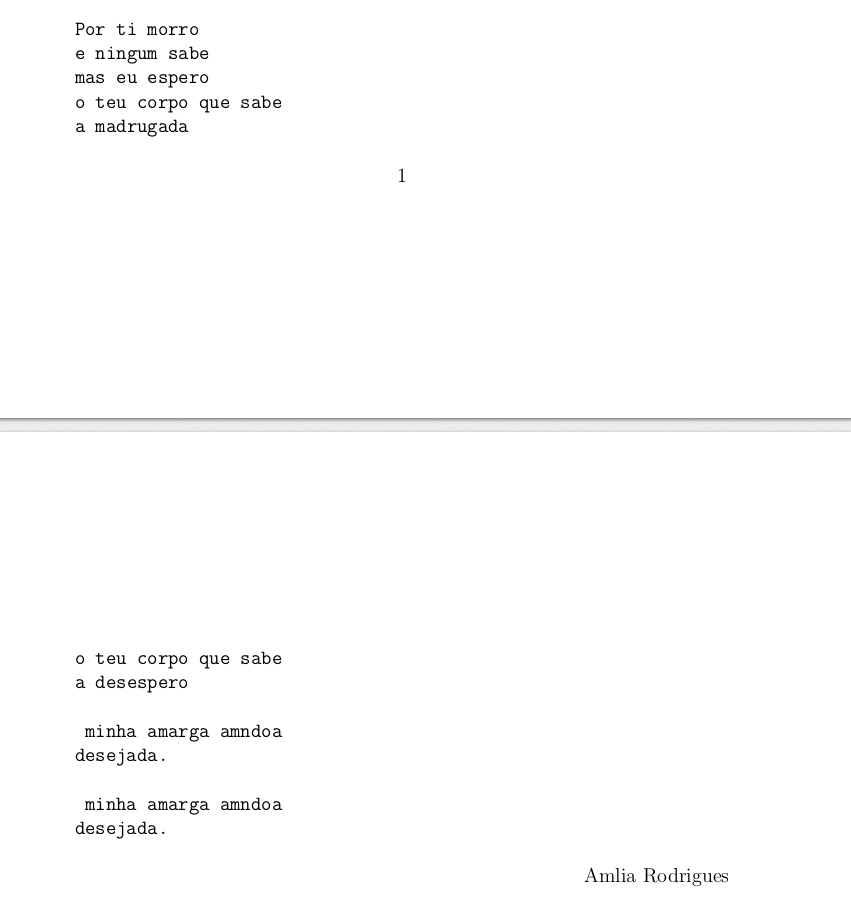
\includegraphics[width=15cm]{anexos/2-5/2-5-a-img2.png}
\caption{PDF gerado por o ficheiro latex (teste 1). Pagina 2 de 2}
\label{fig::anex-music-test-img}
\end{figure}

\begin{figure}
\centering
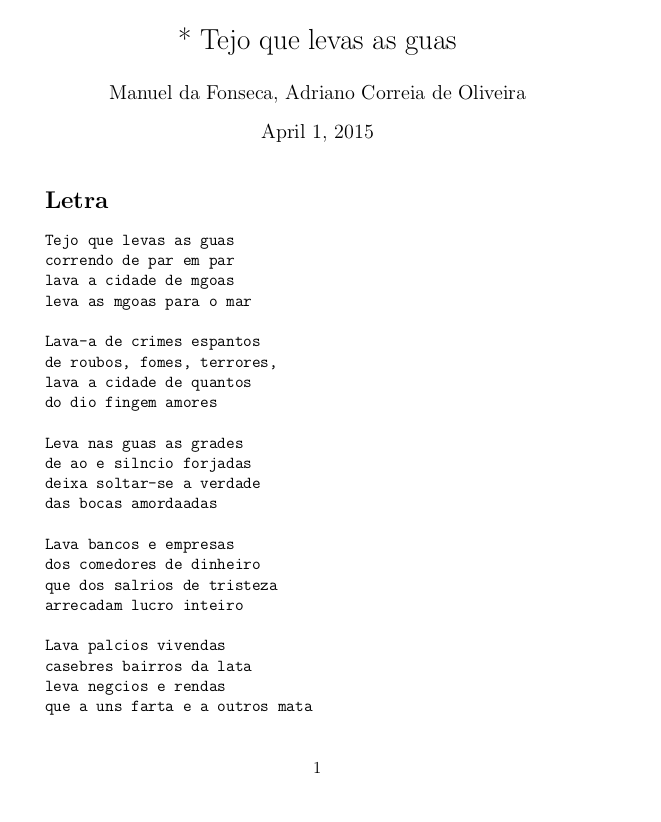
\includegraphics[width=15cm]{anexos/2-5/2-5-b-img.png}
\caption{PDF gerado por o ficheiro latex (teste 2). Pagina 1 de 2}
\label{fig::anex-music-test-img02}
\end{figure}

\begin{figure}
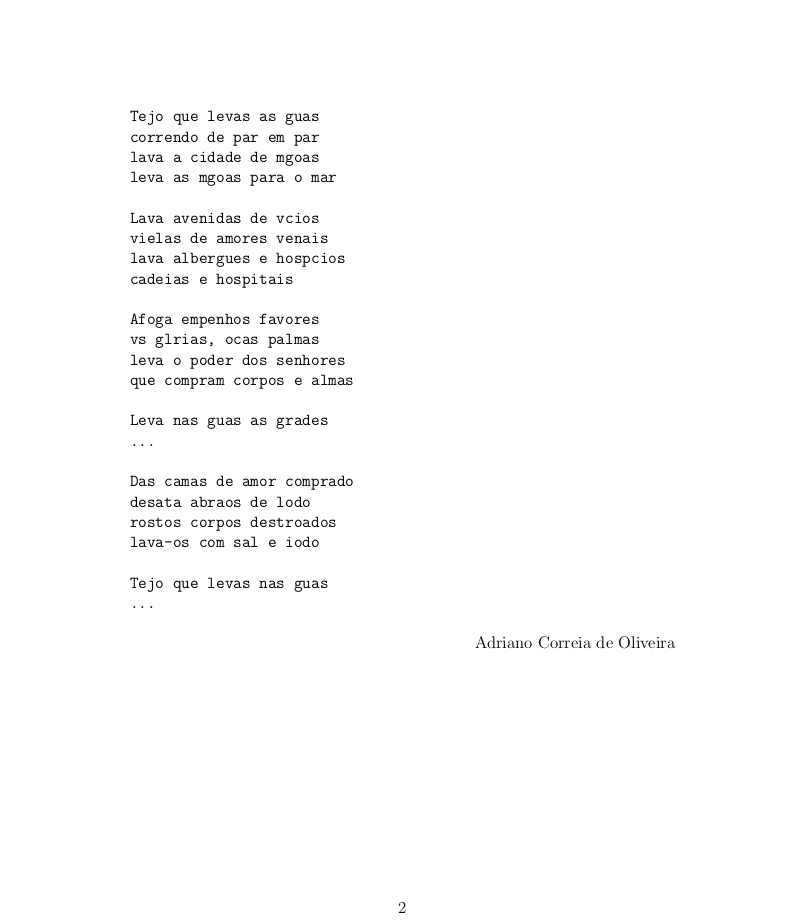
\includegraphics[width=15cm]{anexos/2-5/2-5-b-img2.png}
\caption{PDF gerado por o ficheiro latex (teste 2). Pagina 2 de 2}
\label{fig::anex-music-test-img}
\end{figure}

\begin{figure}
\centering
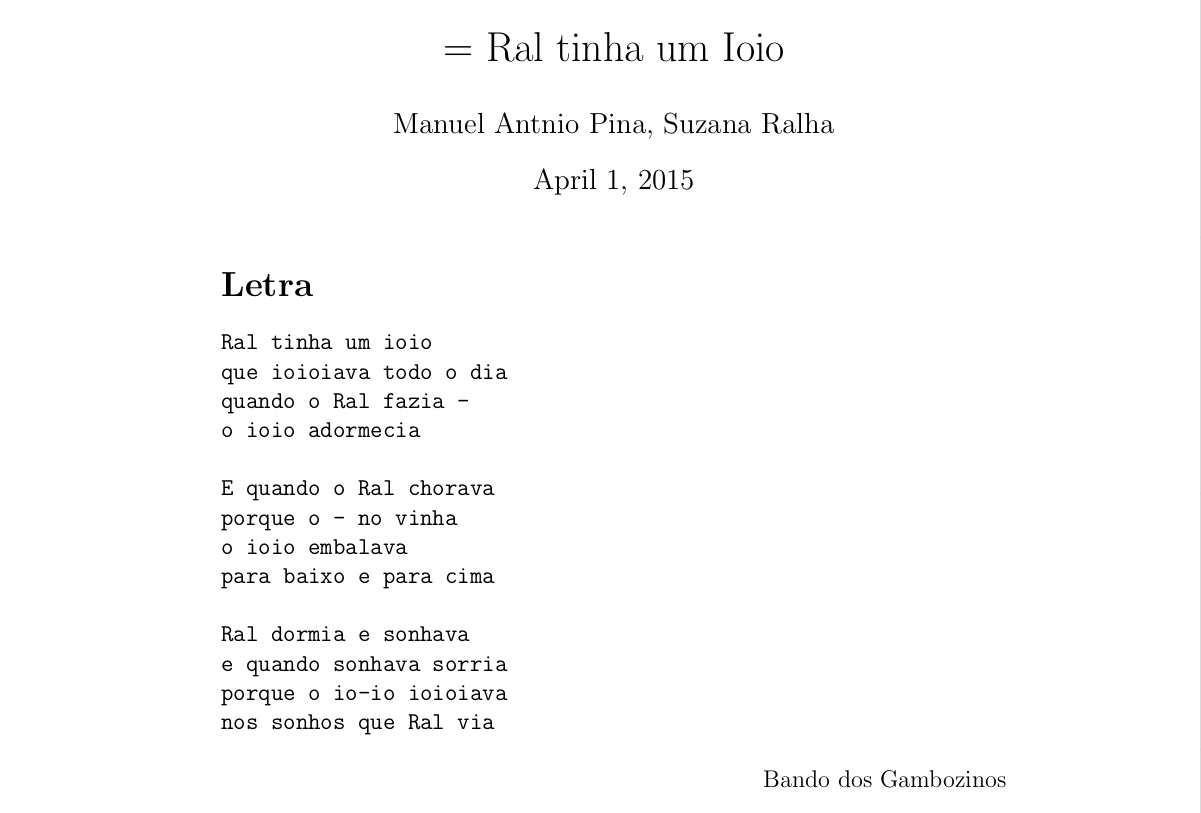
\includegraphics[width=15cm]{anexos/2-5/2-5-c-img.png}
\caption{PDF gerado por o ficheiro latex (teste 3)}
\label{fig::anex-music-test-img03}
\end{figure}
\end{document}


% respectivo enunciado, da descricao do problema, das decisoes que lideraram o desenho da solucao e sua implementacao (incluir a especificacao Flex , deverao conter exemplos de utilizacao (textos fontes diversos e respectivo resultado produzido)